% !TeX root = quantum-mechanics.tex

\documentclass[english,course]{lecture}
\usepackage{amsmath}
\usepackage{graphicx}
\usepackage{float}
\usepackage{hyperref}

% Document metadata
\title{Knowledge Base}
\subtitle{Quantum Mechanics: Amplitudes, Waves, and Spin}
\shorttitle{Quantum mechanics}
\subject{Biophysics}
\author{Alex Payne}
\email{alex.payne@choderalab.org}
\attn{The ideas behind the wave function, energy and momentum, and why the electron is a fermion}
\morelink{http://choderalab.org}
%
% Begin document
\begin{document}

\vfill
\eject

%%%%%%%%%%%%%%%%%%%%%%%%%%%%%%%%%%%%%%%%%%%%%%%%%%%%%%%%%%%%%%%%%%%%%%%%%%%%%%%%%%%%%%%%%%%%%%%%%%%%%%%%%%%%%%%%%%%%%%%%%%%%%%%%%%%%
%% READING
%%%%%%%%%%%%%%%%%%%%%%%%%%%%%%%%%%%%%%%%%%%%%%%%%%%%%%%%%%%%%%%%%%%%%%%%%%%%%%%%%%%%%%%%%%%%%%%%%%%%%%%%%%%%%%%%%%%%%%%%%%%%%%%%%%%%

\section{Recommended reading and supportive texts}

\subsection*{Recommended reading}

\noindent {\bf The Feynman Lectures on Physics, Vol.~III: Quantum Mechanics}, Feynman, Leighton, and Sands \\
The source for most of what follows. Chapters 1 (quantum behavior), 6 (spin one-half), 7 (amplitudes in time), 16 (amplitudes in position), and 17 (symmetry and conservation laws). The online edition is free and uses the same chapter, section, and equation numbers as the printed one.
\href{https://www.feynmanlectures.caltech.edu/III_toc.html}{[Online edition]}

\subsection*{Optional reading and supportive texts}

% TODO: add a standard graduate text (e.g.\ Sakurai or Griffiths) and a text on quantum chemistry (Szabo--Ostlund) once the electronic-structure notes exist.

\vfill
\eject

%%%%%%%%%%%%%%%%%%%%%%%%%%%%%%%%%%%%%%%%%%%%%%%%%%%%%%%%%%%%%%%%%%%%%%%%%%%%%%%%%%%%%%%%%%%%%%%%%%%%%%%%%%%%%%%%%%%%%%%%%%%%%%%%%%%%
%% INTRODUCTION
%%%%%%%%%%%%%%%%%%%%%%%%%%%%%%%%%%%%%%%%%%%%%%%%%%%%%%%%%%%%%%%%%%%%%%%%%%%%%%%%%%%%%%%%%%%%%%%%%%%%%%%%%%%%%%%%%%%%%%%%%%%%%%%%%%%%

\section{Why quantum mechanics, and what these notes cover}

Quantum mechanics is the most accurate description we have of the electrons that hold molecules together. It is the reference that force fields are trained against (see the force fields notes), the theory behind every electronic-structure method (Hartree--Fock, DFT, coupled cluster), and the reason atoms have shells and chemistry has a periodic table.

These notes are not a survey of methods. They collect a small set of ideas that the rest of the subject is built on, developed from the smallest possible starting point and assuming only trigonometry (complex numbers are introduced when needed):

\begin{itemize}
    \item \textbf{Amplitudes}: the state of a system is a list of complex numbers; probabilities are their squared sizes; phases matter only when amplitudes are combined.
    \item \textbf{Waves}: waves add by arrows, and a state of definite energy and momentum is a plane wave $e^{i(kx-\omega t)}$, and $E=\hbar\omega$, $p=\hbar k$ say that energy and momentum are its rotation rates in time and in space.
    \item \textbf{Symmetry and conservation}: if the physics is unchanged by a shift or a rotation, the corresponding phase rate is conserved. This is Noether's theorem in quantum form.
    \item \textbf{Spin}: what rotation symmetry says about angular momentum, why the electron has two spin states, and why a rotation through $2\pi$ changes the sign of its state.
    \item \textbf{Fermions and bosons}: which of these facts are consequences of rotation symmetry and which need more (the spin-statistics theorem).
\end{itemize}

Most of this material was worked out in two interactive notebooks (\texttt{spinor\_rotation.py} and \texttt{plane\_waves\_and\_packets.py}, built with marimo) and is summarized here with the key equations. Units are those of the text unless stated; $\hbar=h/2\pi$ is Planck's constant divided by $2\pi$.

%%%%%%%%%%%%%%%%%%%%%%%%%%%%%%%%%%%%%%%%%%%%%%%%%%%%%%%%%%%%%%%%%%%%%%%%%%%%%%%%%%%%%%%%%%%%%%%%%%%%%%%%%%%%%%%%%%%%%%%%%%%%%%%%%%%%
%% WAVES (TRIGONOMETRIC)
%%%%%%%%%%%%%%%%%%%%%%%%%%%%%%%%%%%%%%%%%%%%%%%%%%%%%%%%%%%%%%%%%%%%%%%%%%%%%%%%%%%%%%%%%%%%%%%%%%%%%%%%%%%%%%%%%%%%%%%%%%%%%%%%%%%%

\section{Waves in trigonometric form}
\label{sec:waves}

Quantum amplitudes behave like waves, so we start with an ordinary wave, such as the height of the surface of water, written with a cosine. Every such wave is built from one function, so we start with that function alone, and then describe the wave in three steps: how it varies in time at one position, how it varies in space at one moment, and then both together.

\subsection{The phase}
\label{sec:phase}

Consider
\[
H(\theta)=A\cos\theta,
\]
where $\theta$ is an angle in radians. The angle $\theta$ is called the \textbf{phase}: it says how far through its cycle the cosine has got. At $\theta=0$ the cosine is at a crest ($H=A$), at $\theta=\pi/2$ it crosses zero on the way down, at $\theta=\pi$ it is at a trough ($H=-A$), and at $\theta=2\pi$ it is back at the crest. The cosine therefore repeats whenever the phase grows by $2\pi$. The amplitude $A$ is the largest height; the phase decides where in the cycle the height is. The same value can be pictured as an arrow of length $A$ turning on a circle: the phase is the angle of the arrow and $H$ is its horizontal part. This picture returns in section~\ref{sec:complexwaves}.

\begin{figure}[H]
\centering
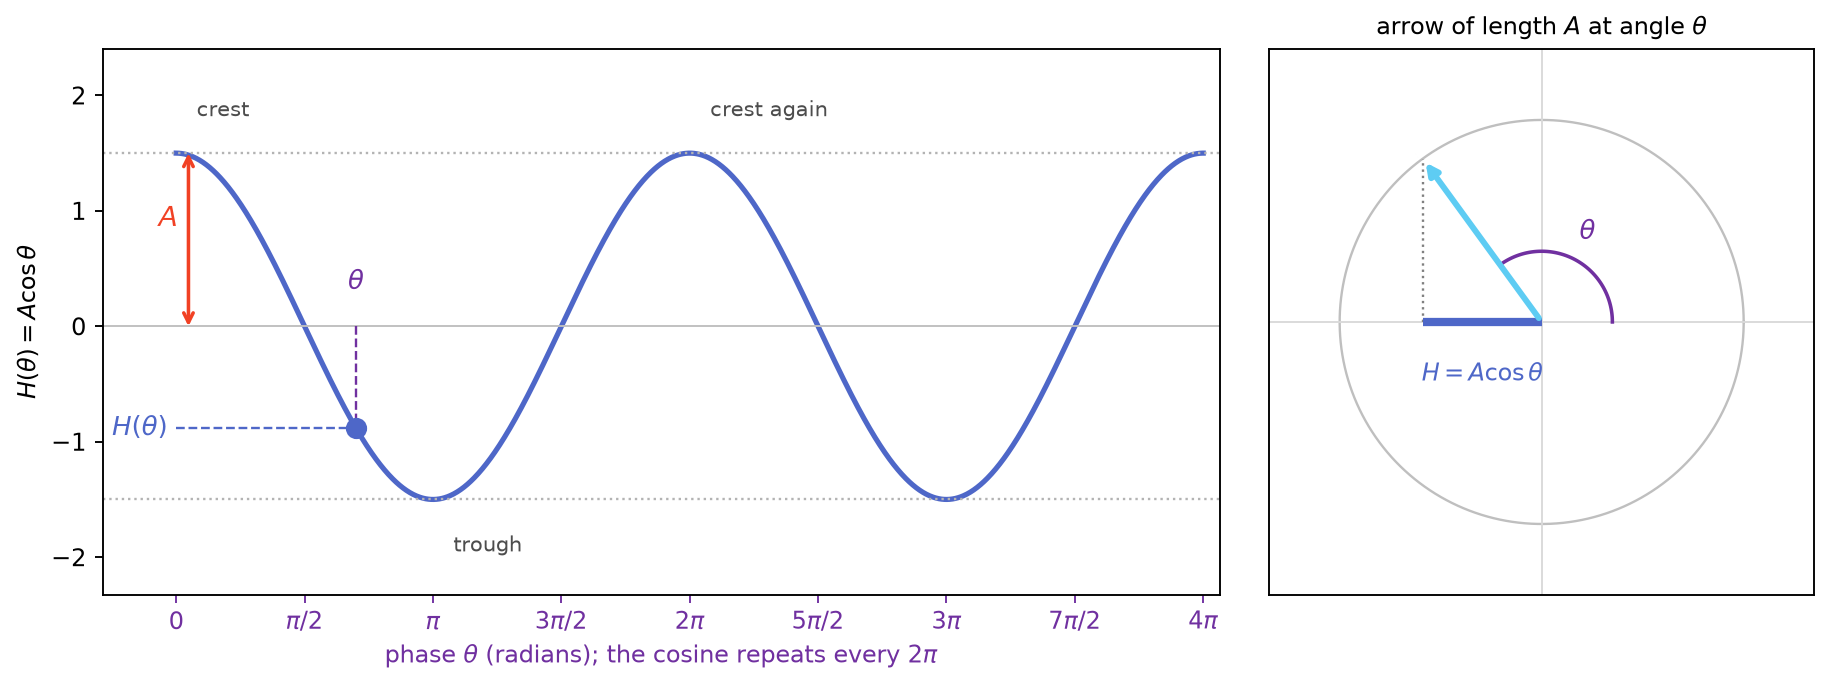
\includegraphics[width=\textwidth]{figures/wave-phase.png}
\caption{The cosine against its phase $\theta$ (left) and the same value as the horizontal part of an arrow of length $A$ at angle $\theta$ (right). The black point on the curve and the black segment on the circle show the same height $H(\theta)$.}
\end{figure}

Everything below is this one function with a particular phase: $\theta=\omega t$ at a fixed position, $\theta=kx$ at a fixed moment, and $\theta=kx-\omega t$ in general.

\subsection{Oscillation in time}

At a fixed position the height oscillates as
\[
H(t)=A\cos(\omega t).
\]
The \textbf{amplitude} $A$ is the largest height reached. The argument of the cosine is now the phase $\theta=\omega t$, which grows by $\omega$ in every unit of time, so $\omega$ is the number of radians covered per unit time: the \textbf{angular frequency}. The cosine repeats when its argument has grown by $2\pi$, after the \textbf{period} $T=2\pi/\omega$; the number of oscillations per unit time is the frequency $f=1/T=\omega/2\pi$.

\begin{figure}[H]
\centering
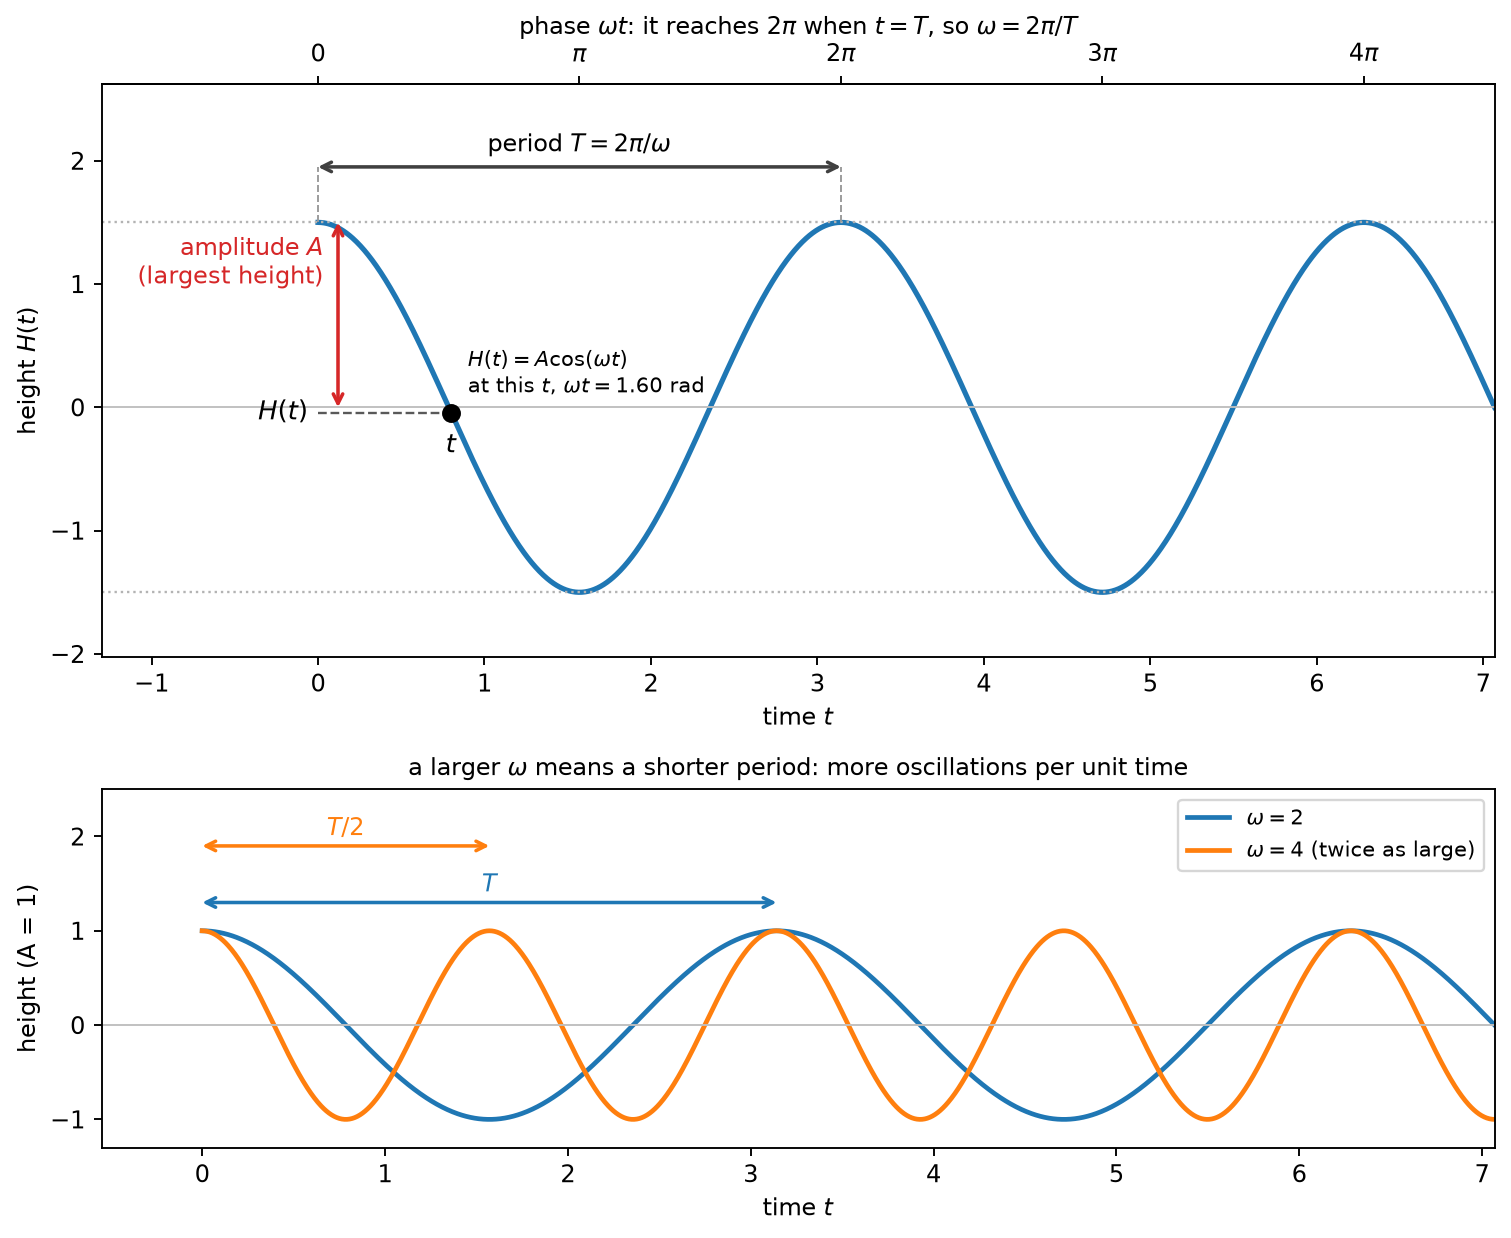
\includegraphics[width=0.82\textwidth]{figures/wave-time-features.png}
\caption{Where each quantity appears on the graph of $H(t)=A\cos(\omega t)$. The amplitude $A$ is a height (red). The period $T$ is the horizontal distance between crests. The time $t$ and the height $H(t)$ are the horizontal and vertical positions of a point on the curve. The angular frequency $\omega$ is not a length: it is the rate at which the phase $\omega t$ (top scale) grows, reaching $2\pi$ at $t=T$, so $\omega=2\pi/T$. Lower panel: doubling $\omega$ halves the period.}
\end{figure}

\subsection{Variation in space}

At a fixed moment the height varies along the line as $H(x)=A\cos(kx)$. The phase is now $\theta=kx$, which grows by $k$ in every unit of distance, so $k$ is the number of radians per unit length: the \textbf{wave number}, the counterpart in space of $\omega$. The cosine repeats after the \textbf{wavelength} $\lambda=2\pi/k$, the counterpart of the period.

\begin{figure}[H]
\centering
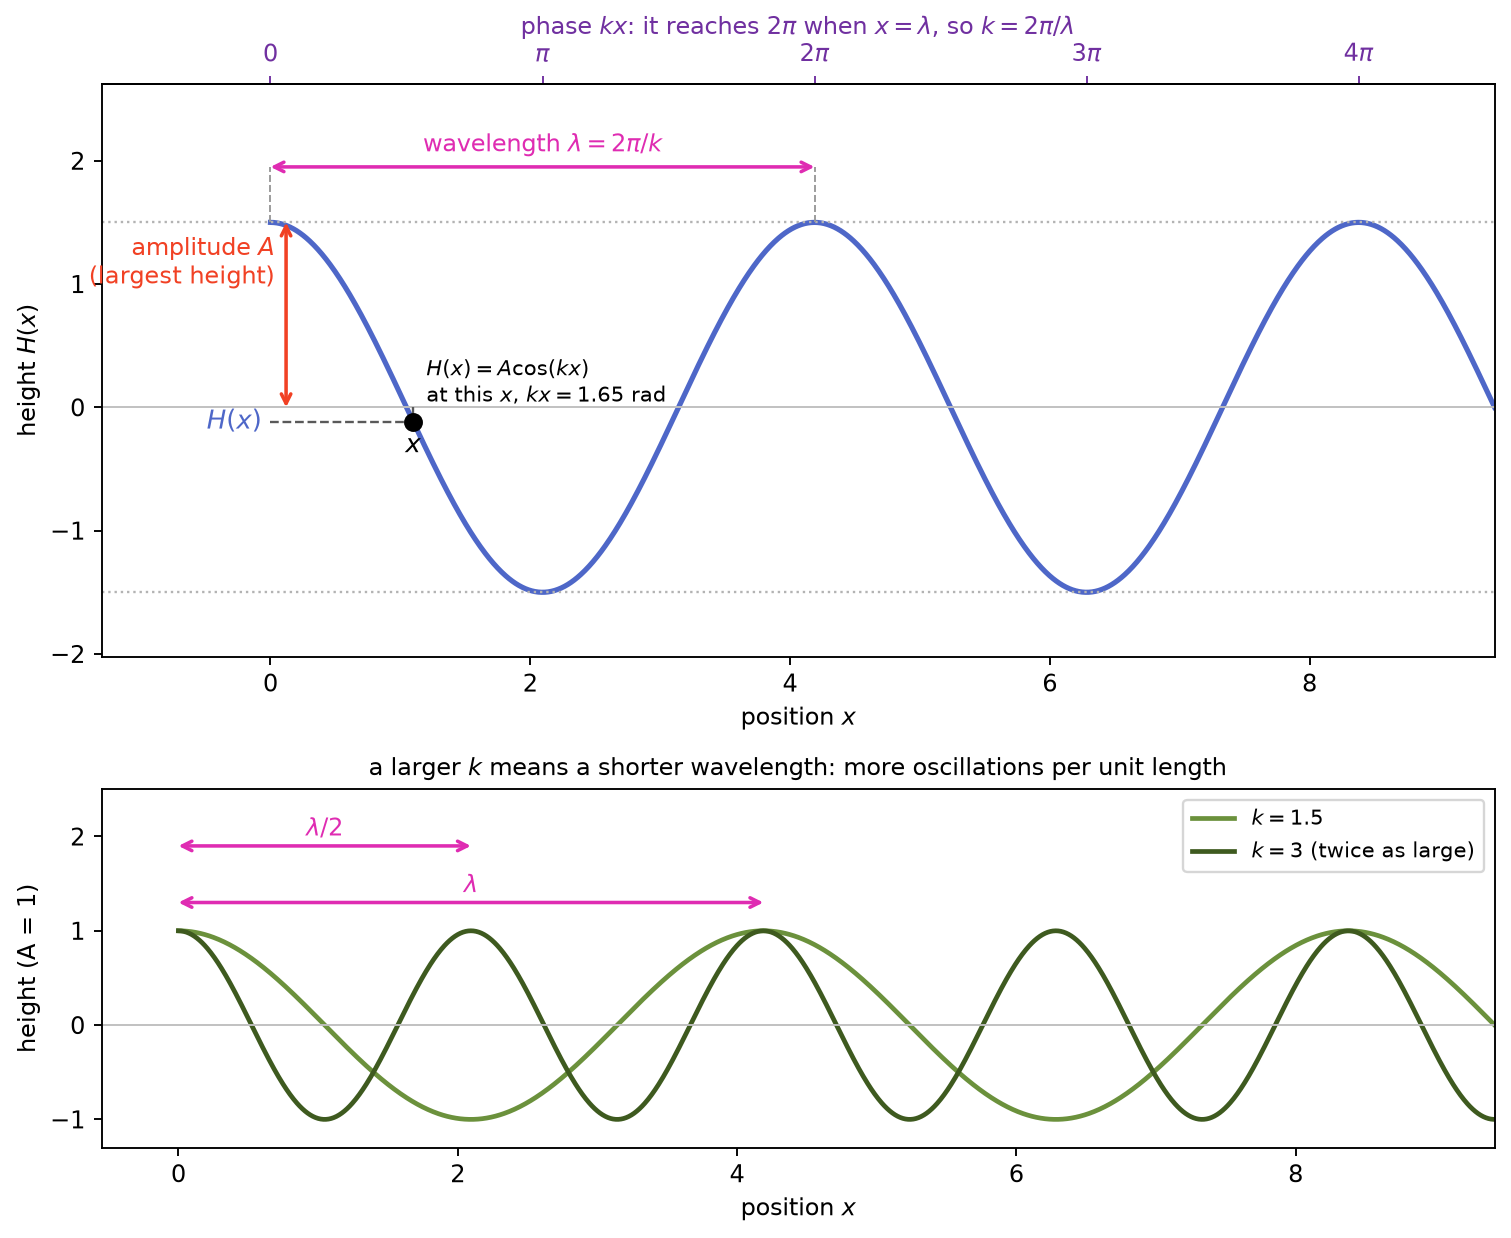
\includegraphics[width=0.82\textwidth]{figures/wave-space-features.png}
\caption{The same graph with position in place of time, for $H(x)=A\cos(kx)$. The wavelength $\lambda$ is a length: the horizontal distance between crests. The wave number $k$ is the rate at which the phase $kx$ (top scale) grows along the line, reaching $2\pi$ at $x=\lambda$, so $k=2\pi/\lambda$. Lower panel: doubling $k$ halves the wavelength.}
\end{figure}

\subsection{A travelling wave}

A wave that varies in both is
\[
H(x,t)=A\cos(kx-\omega t).
\]
The argument $kx-\omega t$ is again the \textbf{phase}, now depending on both position and time. A crest is a point of fixed phase, $kx-\omega t=\text{const}$, so $x=(\omega/k)\,t$ plus a constant, and the whole pattern moves at the \emph{phase velocity}
\[
v_{\text{phase}}=\frac{\omega}{k}=\frac{\lambda}{T}.
\]
This form follows from the motion of a source. If a source at $x=0$ moves as $A\cos(\omega t)$ and the disturbance travels outward at speed $v$, the motion at distance $r$ is that of the source a time $r/v$ earlier, $A\cos(\omega t-kr)$ with $k=\omega/v$, which equals $A\cos(kr-\omega t)$. \textbf{The distance from the source enters only through the phase $kr$}, which increases by $2\pi$ for each further wavelength. Here $r$ is the distance from the source, which plays the role of the position $x$ along the direction in which the wave travels: for a wave moving along a line, $r=x$ and this is $A\cos(kx-\omega t)$. In section~\ref{sec:interference}, $r_1$ and $r_2$ are the distances from two sources (two holes) to a detector, and $x$ is the position of the detector along a line behind the wall. The speed of the pattern is not the speed of a particle (section~\ref{sec:packets}).

\begin{figure}[H]
\centering
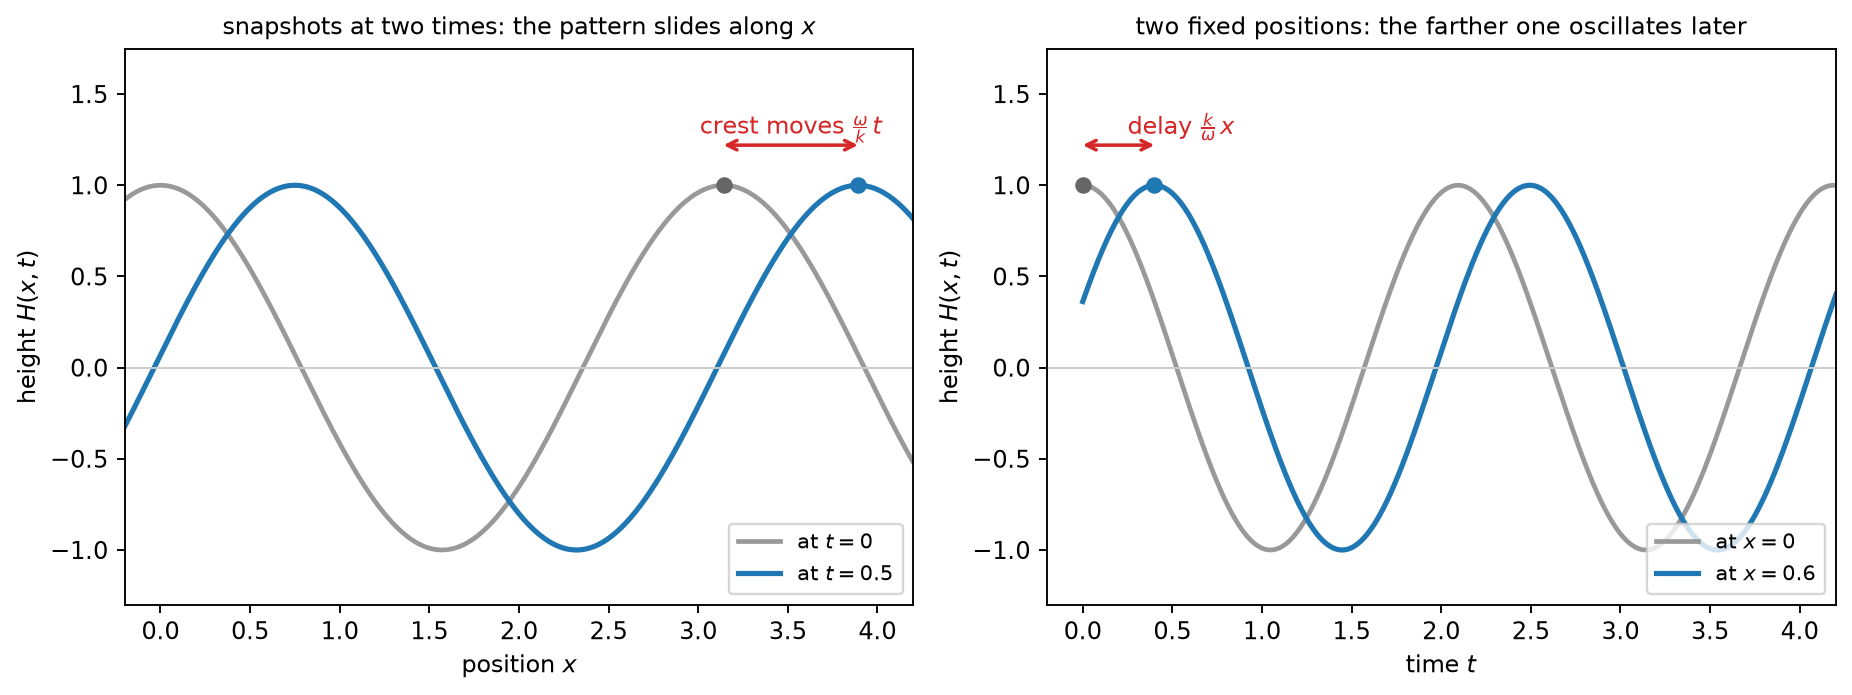
\includegraphics[width=\textwidth]{figures/wave-travelling-features.png}
\caption{Both variables at once, for $H(x,t)=A\cos(kx-\omega t)$. Left: height against position at two times; a crest has moved to the right by $(\omega/k)\,t$. Right: height against time at two fixed positions; the crest reaches the farther position later, after a delay $(k/\omega)\,x$. The space graph and the time graph are two slices of the same wave.}
\end{figure}

\begin{figure}[H]
\centering
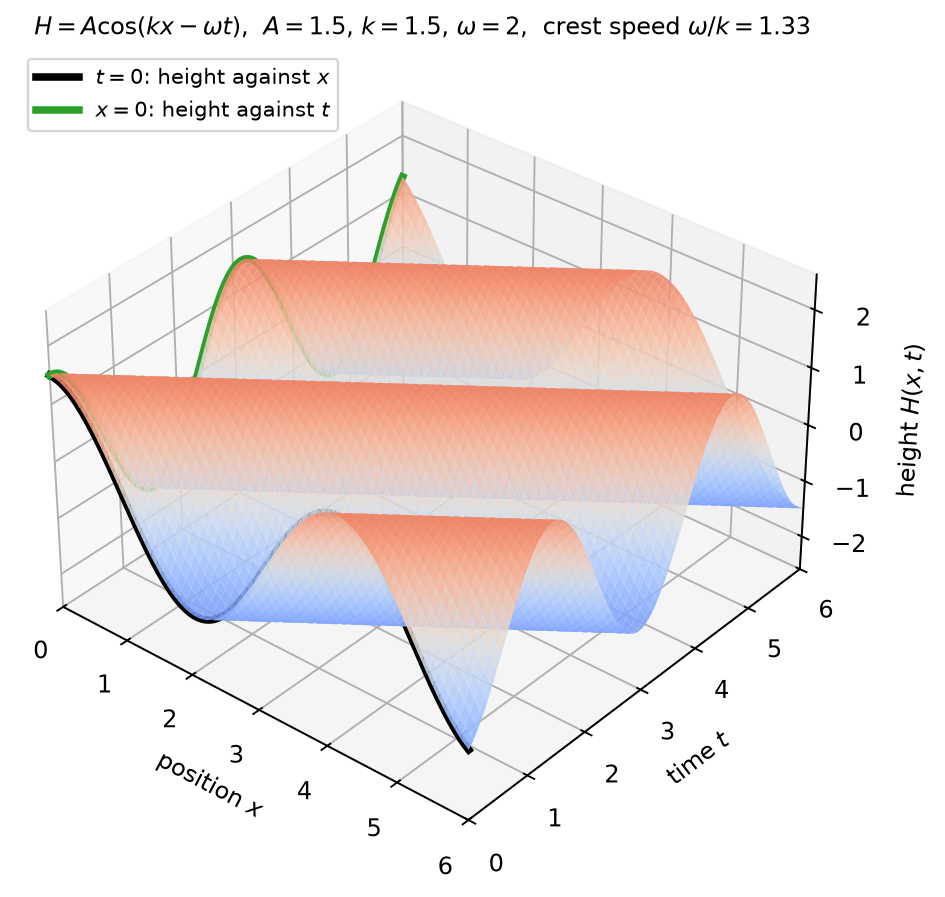
\includegraphics[width=0.9\textwidth]{figures/wave-surface.png}
\caption{The whole wave as a surface, $H(x,t)=A\cos(kx-\omega t)$ with $A=1.5$, $k=1.5$, $\omega=2$. The black curve is the slice $t=0$ (the space graph) and the green curve is the slice $x=0$ (the time graph). The ridges are the crests; they run diagonally because a crest moves along $x$ as $t$ advances, at speed $\omega/k$. Changing $A$ changes the height of the ridges, $k$ their spacing along $x$, and $\omega$ their spacing along $t$.}
\end{figure}

%%%%%%%%%%%%%%%%%%%%%%%%%%%%%%%%%%%%%%%%%%%%%%%%%%%%%%%%%%%%%%%%%%%%%%%%%%%%%%%%%%%%%%%%%%%%%%%%%%%%%%%%%%%%%%%%%%%%%%%%%%%%%%%%%%%%
%% COMPLEX
%%%%%%%%%%%%%%%%%%%%%%%%%%%%%%%%%%%%%%%%%%%%%%%%%%%%%%%%%%%%%%%%%%%%%%%%%%%%%%%%%%%%%%%%%%%%%%%%%%%%%%%%%%%%%%%%%%%%%%%%%%%%%%%%%%%%

\section{The same waves with complex numbers}
\label{sec:complexwaves}

For classical waves such as water, writing the wave with complex numbers is a neat mathematical trick. For quantum amplitudes it becomes necessary (section~\ref{sec:whycomplex}). This section shows that the two descriptions are the same wave.

\subsection{An arrow in the plane}

A complex number $z=a+ib$ can be drawn as an arrow in a plane: $a$ is the horizontal component (real part), $b$ the vertical component (imaginary part). The arrow has a length $|z|$ and points at some angle from the horizontal axis. The arrow of length 1 at angle $\theta$ (in radians) is written
\[
e^{i\theta}=\cos\theta+i\sin\theta,
\]
with horizontal component $\cos\theta$ and vertical component $\sin\theta$. An arrow of length $A$ at the same angle is $A$ times this,
\[
h(\theta)=A\,e^{i\theta}=A\cos\theta+iA\sin\theta .
\]
This is the arrow in the right panel of the figure in section~\ref{sec:phase}, and the angle $\theta$ is the \emph{phase} of that section. Its horizontal component is the cosine of section~\ref{sec:phase},
\[
H(\theta)=A\cos\theta=\operatorname{Re}\,h(\theta),
\]
where $\operatorname{Re}$ means the real part. A notation is fixed here and used from now on: the capital $H$ is the \textbf{real height} of the wave, and the lowercase $h$ is the \textbf{complex} number, the arrow, whose real part is $H$.

\subsection{The real wave is the horizontal component of a turning arrow}

Now replace the phase $\theta$ by the phase of section~\ref{sec:waves}, $\theta=kx-\omega t$. The \textbf{complex wave} is
\[
h(x,t)=A\,e^{i(kx-\omega t)},
\]
and its real part is the wave of section~\ref{sec:waves},
\[
H(x,t)=\operatorname{Re}\,h(x,t)=A\cos(kx-\omega t).
\]
These are equal for every $x$ and $t$: $H$ is the real wave, and $h$ is the arrow of length $A$ at angle $kx-\omega t$ of which $H$ is the horizontal component. The vertical component is $A\sin(kx-\omega t)$, the same wave a quarter of a period later. A wave with a starting phase, $A\cos(kx-\omega t+\theta_0)$, is the real part of $h=a\,e^{i(kx-\omega t)}$ with the \emph{complex amplitude} $a=Ae^{i\theta_0}$, so one complex number holds both the size and the starting phase. The quantities above now have a geometric meaning.

\paragraph{$\omega$ turns the arrow in time.} At a fixed position the arrow is $h(t)=\big(Ae^{ikx}\big)e^{-i\omega t}$. The bracket does not change with time and the phase $-\omega t$ of the second factor grows in proportion to time, so the arrow turns at a steady rate: \textbf{$\omega$ is the number of radians through which it turns per unit time}, and one turn takes the period $T=2\pi/\omega$. (Some texts write $e^{+i\omega t}$, so the arrow turns the other way; that reverses every phase and changes no intensity.)

\paragraph{$k$ twists the arrow in space.} At a fixed time the arrow at position $x$ is $h(x)=\big(Ae^{-i\omega t}\big)e^{ikx}$, so neighboring arrows are turned relative to one another: \textbf{$k$ is the number of radians through which the arrow turns per unit length}, and one turn takes the wavelength $\lambda=2\pi/k$.

Together, the arrow at each position turns in time at rate $\omega$ while neighboring positions are turned at rate $k$, and the crests of its horizontal component move at $\omega/k$. \textbf{Nothing has been added to the description: the real wave and the turning arrow are the same wave written in two ways.}

%%%%%%%%%%%%%%%%%%%%%%%%%%%%%%%%%%%%%%%%%%%%%%%%%%%%%%%%%%%%%%%%%%%%%%%%%%%%%%%%%%%%%%%%%%%%%%%%%%%%%%%%%%%%%%%%%%%%%%%%%%%%%%%%%%%%
%% INTERFERENCE
%%%%%%%%%%%%%%%%%%%%%%%%%%%%%%%%%%%%%%%%%%%%%%%%%%%%%%%%%%%%%%%%%%%%%%%%%%%%%%%%%%%%%%%%%%%%%%%%%%%%%%%%%%%%%%%%%%%%%%%%%%%%%%%%%%%%

\section{Adding waves: interference}
\label{sec:interference}

Waves add when the same medium is disturbed by two sources. Consider water waves in a shallow trough passing through two small holes in a wall. Each hole is a source of circular waves of wavelength $\lambda=2\pi/k$ and angular frequency $\omega$. A detector on the far side measures the intensity of the wave motion, proportional to the average of the square of the height. It sits at distance $r_1$ from hole~1 and $r_2$ from hole~2. (These are distances from each hole to the detector, as in section~\ref{sec:waves}, not the position $x$ of the detector along the line behind the wall, which appears in the figure.)

The calculation goes in steps, from the complex waves to the real height.

\paragraph{Step 1: one complex wave for each hole.} By section~\ref{sec:waves} the real height at the detector from hole~1 is $H_1(t)=A_1\cos(kr_1-\omega t)$, with $A_1$ the size of the wave at the detector. Its complex wave, in the notation of section~\ref{sec:complexwaves}, is
\[
h_1(t)=A_1e^{i(kr_1-\omega t)},\qquad H_1(t)=\operatorname{Re}\,h_1(t).
\]
The direction of this arrow is the phase $kr_1-\omega t$: the part $kr_1$ is set by the distance from the hole (one more wavelength turns it by $2\pi$) and the part $-\omega t$ turns the arrow in time. Hole~2 gives $h_2(t)=A_2e^{i(kr_2-\omega t)}$ and $H_2(t)=\operatorname{Re}\,h_2(t)$.

\paragraph{Step 2: add the complex waves.}
\[
h_{12}(t)=h_1(t)+h_2(t).
\]

\paragraph{Step 3: the real part is the real height.} The real part of a sum is the sum of the real parts, so
\[
\operatorname{Re}\,h_{12}(t)=\operatorname{Re}\,h_1(t)+\operatorname{Re}\,h_2(t)=H_1(t)+H_2(t)=H_{12}(t).
\]
This is the height of the water with both holes open, since the heights add. Adding the arrows and then taking the real part gives the same wave as adding the real waves.

\paragraph{Step 4: separate the part that turns.} Both arrows contain the factor $e^{-i\omega t}$, so
\[
h_{12}(t)=\big(A_1e^{ikr_1}+A_2e^{ikr_2}\big)\,e^{-i\omega t}.
\]
The bracket is the sum of the two arrows at $t=0$ (top left of the figure below), placed tip to tail. The factor $e^{-i\omega t}$ turns the whole sum, and the two arrows keep the same angle $\delta=k(r_2-r_1)$ between them, so the \emph{length} of the sum does not change in time.

\paragraph{Step 5: the intensity is the squared length.} For a wave $H=\operatorname{Re}[c\,e^{-i\omega t}]$ the average of $H^2$ over a period is $\tfrac12|c|^2$. The constant $\tfrac12$ is the same for every wave and is dropped, so the intensity is $I=|h|^2$. Since $|e^{-i\omega t}|=1$, the intensity of one hole is $I_1=|h_1|^2=A_1^2$, and with both holes open
\[
I_{12}=|h_{12}|^2=\big|A_1e^{ikr_1}+A_2e^{ikr_2}\big|^2=A_1^2+A_2^2+2A_1A_2\cos\delta .
\]
The last step uses $|u+v|^2=|u|^2+|v|^2+2\operatorname{Re}(u^*v)$ with $u^*v=A_1A_2e^{i\delta}$. In terms of the single-hole intensities,
\[
I_{12}=I_1+I_2+2\sqrt{I_1I_2}\,\cos\delta .
\]
The last term is the interference term, and $\delta$ is the angle between the two arrows: parallel arrows add their lengths, opposite arrows subtract them. For two waves of equal size, $I_{12}$ is largest, four times the intensity of one wave, where $\delta$ is a multiple of $2\pi$ (the distances differ by whole wavelengths), and zero where $\delta$ is an odd multiple of $\pi$ (the distances differ by an odd number of half-wavelengths). The result is not $I_1+I_2$: the waves \emph{interfere}. For waves of unequal size, or any number of waves, the arrows are simply placed tip to tail, with no extra work.\footnote{The same result in trigonometric form, for two waves of equal size $A$. The heights are $H_1=A\cos(kr_1-\omega t)$ and $H_2=A\cos(kr_2-\omega t)$, and the identity $\cos a+\cos b=2\cos\frac{a-b}{2}\cos\frac{a+b}{2}$ gives $H_{12}(t)=2A\cos\frac{\delta}{2}\cos\!\big(\frac{k(r_1+r_2)}{2}-\omega t\big)$. This is a wave of the same frequency whose size is $2A|\cos(\delta/2)|$, so $I_{12}=4A^2\cos^2(\delta/2)$. The arrows give the same: with $A_1=A_2=A$, $I_{12}=2A^2+2A^2\cos\delta=4A^2\cos^2(\delta/2)$. For unequal sizes, or for three or more waves, the identity no longer applies directly and the algebra grows quickly, whereas arrows keep adding.}

\begin{figure}[ht]
\centering
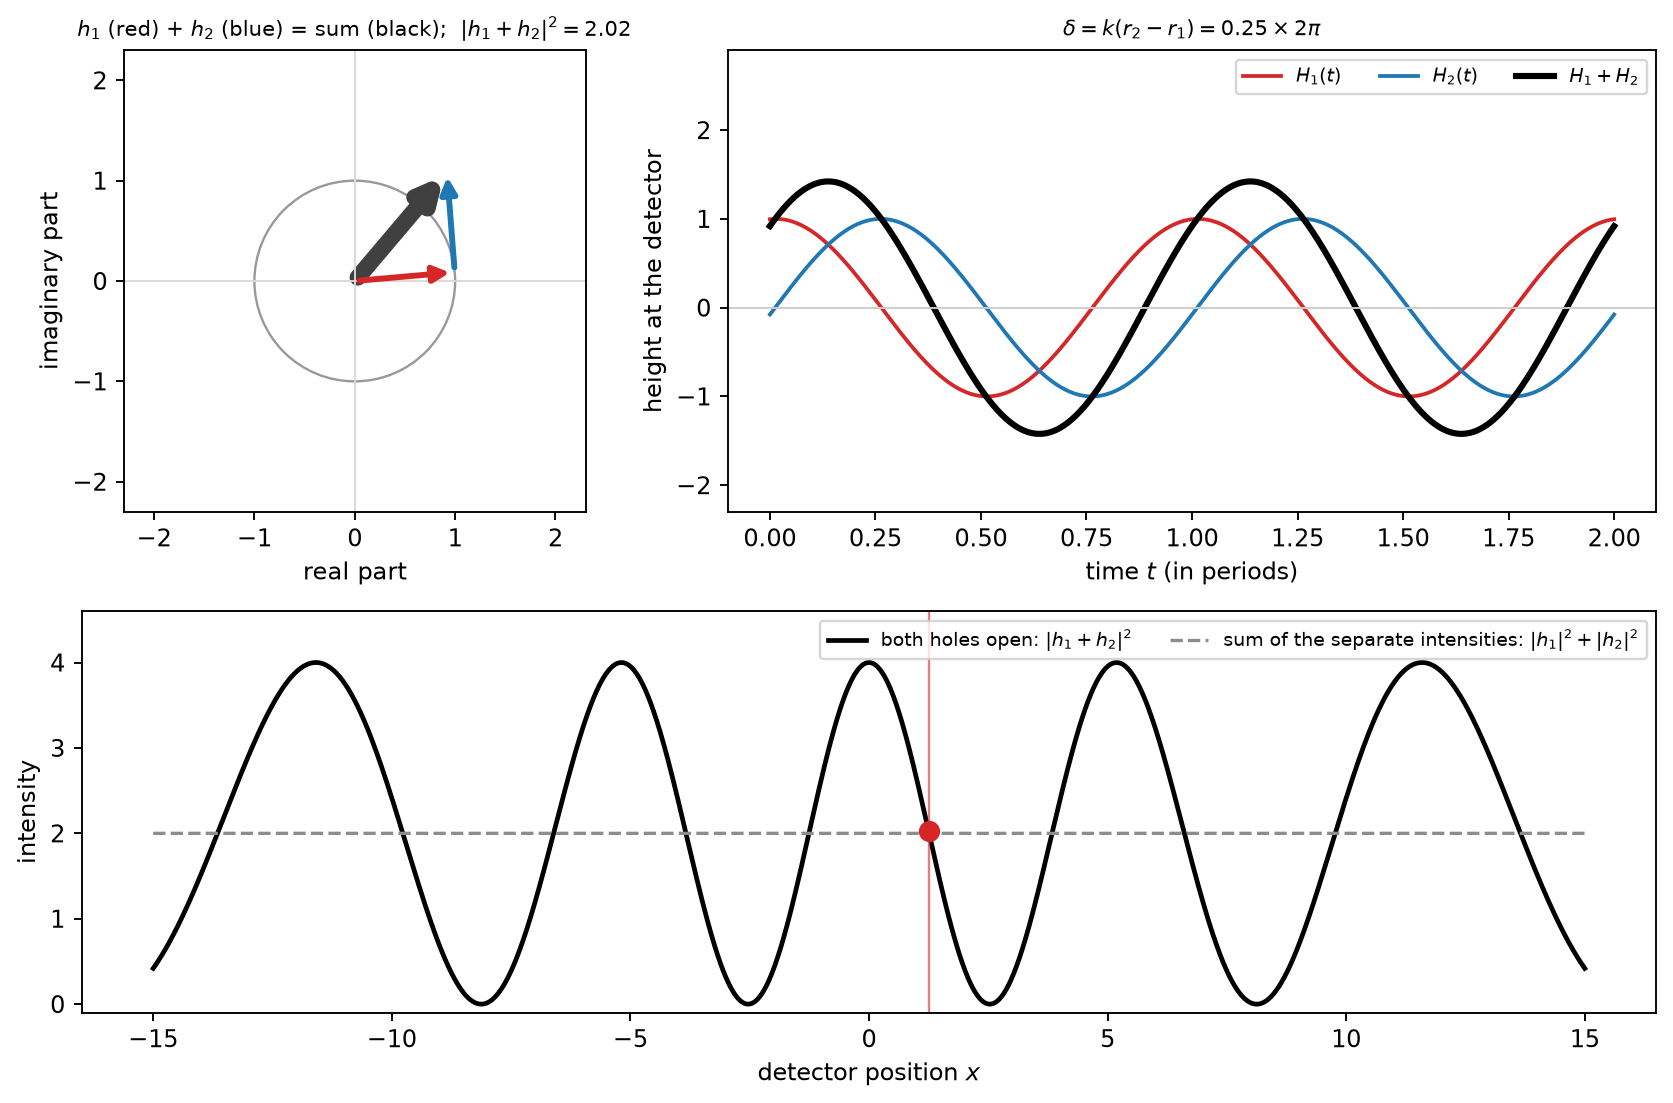
\includegraphics[width=\textwidth]{figures/two-hole-interference.png}
\caption{Two holes $d=4$ apart, $\lambda=1$, detector line 20 units behind the wall. Top left: the arrows $h_1$ (red) and $h_2$ (blue) tip to tail, and their sum (black), at $t=0$ and at the detector position marked in the bottom panel. Top right: the real heights over two periods. Bottom: intensity along the detector line; dashed is $I_1+I_2$, the intensity if the waves did not interfere.}
\end{figure}

%%%%%%%%%%%%%%%%%%%%%%%%%%%%%%%%%%%%%%%%%%%%%%%%%%%%%%%%%%%%%%%%%%%%%%%%%%%%%%%%%%%%%%%%%%%%%%%%%%%%%%%%%%%%%%%%%%%%%%%%%%%%%%%%%%%%
%% WHY COMPLEX
%%%%%%%%%%%%%%%%%%%%%%%%%%%%%%%%%%%%%%%%%%%%%%%%%%%%%%%%%%%%%%%%%%%%%%%%%%%%%%%%%%%%%%%%%%%%%%%%%%%%%%%%%%%%%%%%%%%%%%%%%%%%%%%%%%%%

\section{Why the waves must be complex for quantum amplitudes}
\label{sec:whycomplex}

For classical waves such as water, the height is real and the complex number is only a neat way to add waves: a real cosine would do, with more algebra. For a particle the situation is different, and the complex form is necessary.

\paragraph{Uniform probability.} The amplitude $e^{i(kx-\omega t)}$ has length 1 everywhere and at all times, so the probability of finding the particle is uniform and constant. This is the correct description of a state of definite energy and momentum: the momentum is exactly known, so the position is completely undetermined. A real wave such as $\cos(kx-\omega t)$ would not do, because its square has nodes (positions of zero probability) and oscillates in time. The complex form avoids both because its length does not change as the arrow turns.

\paragraph{The quantum rule.} The rule for adding arrows (section~\ref{sec:interference}) holds for these amplitudes as well. If $\phi_1$ and $\phi_2$ are the amplitudes for a particle to arrive at a detector through hole~1 and through hole~2, the probability with both holes open is $|\phi_1+\phi_2|^2$ and not $|\phi_1|^2+|\phi_2|^2$. Here the complex number \emph{is} the amplitude, and its real part alone would not give the right interference.

%%%%%%%%%%%%%%%%%%%%%%%%%%%%%%%%%%%%%%%%%%%%%%%%%%%%%%%%%%%%%%%%%%%%%%%%%%%%%%%%%%%%%%%%%%%%%%%%%%%%%%%%%%%%%%%%%%%%%%%%%%%%%%%%%%%%
%% AMPLITUDES
%%%%%%%%%%%%%%%%%%%%%%%%%%%%%%%%%%%%%%%%%%%%%%%%%%%%%%%%%%%%%%%%%%%%%%%%%%%%%%%%%%%%%%%%%%%%%%%%%%%%%%%%%%%%%%%%%%%%%%%%%%%%%%%%%%%%

\section{Amplitudes, probabilities, and phase}
\label{sec:amplitudes}

\subsection{Probabilities from amplitudes}

The state of a quantum system is described by one or more complex numbers, called \emph{amplitudes}. The probability of an outcome is the squared length of its amplitude,
\[
P=|a|^2.
\]
Writing $a=|a|e^{i\varphi}$, the phase $\varphi$ does not enter $P$. In particular, $a$ and $-a$ give the same probability.

\subsection{Phases matter when amplitudes are combined}

If a particle can reach a detector by two routes, the amplitudes are added \emph{before} squaring (section~\ref{sec:interference}). For two routes of equal weight with amplitudes $a_1=1$ and $a_2=e^{i\varphi}$,
\[
P=\left|\frac{a_1+a_2}{2}\right|^2=\cos^2\!\left(\frac{\varphi}{2}\right).
\]
The routes reinforce at $\varphi=0$ ($P=1$) and cancel at $\varphi=\pi$, that is for $a_2=-1$ ($P=0$), although $|a_2|^2=1$ in both cases. A sign that changes no probability on its own can therefore be detected by interference with an unchanged copy. This single observation underlies the strange behavior of spin in section~\ref{sec:spinhalf}.

\subsection{Overall phase is unobservable}

Multiplying \emph{all} amplitudes of a state by the same phase changes no probability, and no interference between parts of that state. Only relative phases are physical. Consequently, adding a constant to every energy changes nothing observable (it multiplies every amplitude by the same turning arrow); only energy \emph{differences} matter.

\subsection{An example: the hydrogen molecular ion}

Two protons share one electron. Write the state as $(a_1,a_2)$, the amplitudes to find the electron near proton 1 or proton 2. Reflecting the system in the plane halfway between the protons turns $(a_1,a_2)$ into $(a_2,a_1)$. The state $\tfrac{1}{\sqrt2}(1,1)$ is unchanged; the state $\tfrac{1}{\sqrt2}(1,-1)$ becomes $\tfrac{1}{\sqrt2}(-1,1)$, which is minus itself. All probabilities are the same before and after, yet the second state has had its sign reversed. Two reflections restore any state, so a reflection can multiply a state only by $+1$ or $-1$. The same argument returns for the exchange of identical particles (section~\ref{sec:statistics}).

%%%%%%%%%%%%%%%%%%%%%%%%%%%%%%%%%%%%%%%%%%%%%%%%%%%%%%%%%%%%%%%%%%%%%%%%%%%%%%%%%%%%%%%%%%%%%%%%%%%%%%%%%%%%%%%%%%%%%%%%%%%%%%%%%%%%
%% ENERGY AND MOMENTUM
%%%%%%%%%%%%%%%%%%%%%%%%%%%%%%%%%%%%%%%%%%%%%%%%%%%%%%%%%%%%%%%%%%%%%%%%%%%%%%%%%%%%%%%%%%%%%%%%%%%%%%%%%%%%%%%%%%%%%%%%%%%%%%%%%%%%

\section{Energy and momentum are these rates}
\label{sec:planewaves}


The physical content is in two relations,
\[
E=\hbar\omega,\qquad p=\hbar k .
\]
Energy is the rotation rate in time; momentum is the rotation rate in space. The wavelength is therefore $\lambda=2\pi/k=h/p$ (the de~Broglie relation).

\paragraph{Where they come from.} Both have the same origin as the conservation laws. Suppose the physical situation is unchanged by a shift in position, as in empty space. A plane wave $e^{ikx}$ is then a state that a shift only multiplies by a phase, proportional to the size of the shift, whose rate is $k$. A phase factor of this kind cannot change as time passes, so the rate $k$ is conserved: this is the quantum form of conservation of momentum. The same argument for shifts in time gives conservation of energy, with rate $\omega$. The constant $\hbar$ converts these rates to the momentum and energy of classical mechanics, to which they must agree for large systems; its value is fixed by experiment.

\paragraph{Why one constant serves both.} Relativity requires it: energy and momentum are the time part and space part of one four-vector, and so are frequency and wave number. A particle at rest has the pure time rotation $e^{-iE_0t/\hbar}$. An observer who sees it moving with speed $v$ uses the Lorentz-transformed time $t=\gamma(t'-vx'/c^2)$ and finds $E_0t=E't'-p'x'$ with $E'=\gamma E_0$ and $p'=E'v/c^2$, so the amplitude is $e^{-i(E't'-p'x')/\hbar}$, with $\omega=E'/\hbar$ and $k=p'/\hbar$.

\paragraph{Free particle dispersion.} For a slow particle of mass $m$, $E=p^2/2m$, so
\[
\omega(k)=\frac{\hbar k^2}{2m}.
\]

%%%%%%%%%%%%%%%%%%%%%%%%%%%%%%%%%%%%%%%%%%%%%%%%%%%%%%%%%%%%%%%%%%%%%%%%%%%%%%%%%%%%%%%%%%%%%%%%%%%%%%%%%%%%%%%%%%%%%%%%%%%%%%%%%%%%
%% WAVE PACKETS
%%%%%%%%%%%%%%%%%%%%%%%%%%%%%%%%%%%%%%%%%%%%%%%%%%%%%%%%%%%%%%%%%%%%%%%%%%%%%%%%%%%%%%%%%%%%%%%%%%%%%%%%%%%%%%%%%%%%%%%%%%%%%%%%%%%%

\section{Wave packets: when a lump moves like a particle}
\label{sec:packets}

A single plane wave has the same probability everywhere, so it cannot describe a particle that is \emph{somewhere}. A localized particle is a superposition of plane waves with wave numbers close to $k_0$:
\[
\psi(x,t)=\sum_k a(k)\,e^{i(kx-\omega(k)t)}.
\]
Where the waves are in step their amplitudes add; elsewhere they cancel, leaving a lump. The weights $a(k)$ are \emph{amplitudes} with a common phase (a coherent superposition), not Boltzmann-type probabilities (which would give an incoherent mixture and no lump).

\subsection{Uncertainty}

Take $a(k)$ to be a bell curve centered on $k_0$ with root-mean-square width $\sigma_k$, all components in phase at $x=0$ when $t=0$. Then $|\psi(x,0)|^2$ is also a bell curve, with width $\sigma_x$, and
\[
\sigma_x\sigma_k=\tfrac12,\qquad\text{that is}\qquad \Delta x\,\Delta p=\frac{\hbar}{2},
\]
with $\Delta x=\sigma_x$ and $\Delta p=\hbar\sigma_k$. This is the uncertainty principle: a property of the state, not a measurement error. The bell curve (Gaussian) is the shape that makes the product as small as possible. A narrow lump in position requires a broad range of $k$, and the reverse.

\subsection{The lump moves at the classical velocity}

Expand the rotation rate about $k_0$:
\[
\omega(k)=\omega_0+v\,(k-k_0)+\frac{\hbar}{2m}(k-k_0)^2,\qquad v=\frac{d\omega}{dk}\Big|_{k_0}=\frac{\hbar k_0}{m}=\frac{p_0}{m}.
\]
The linear term turns $x$ into $x-vt$ in the sum, so alone it would slide the pattern along unchanged at $v=p_0/m$, the velocity of a classical particle. This lump speed is the \emph{group velocity} $d\omega/dk$, which differs from the crest speed $\omega/k$.

\subsection{The lump spreads}

The quadratic term makes the components fall out of step, and the lump widens. For the Gaussian packet the probability stays a bell curve centered at $x=vt$ with width
\[
\sigma(t)=\sigma_x\sqrt{1+\left(\frac{t}{t_s}\right)^2},\qquad t_s=\frac{2m\sigma_x^2}{\hbar}.
\]

\begin{figure}[h]
\centering
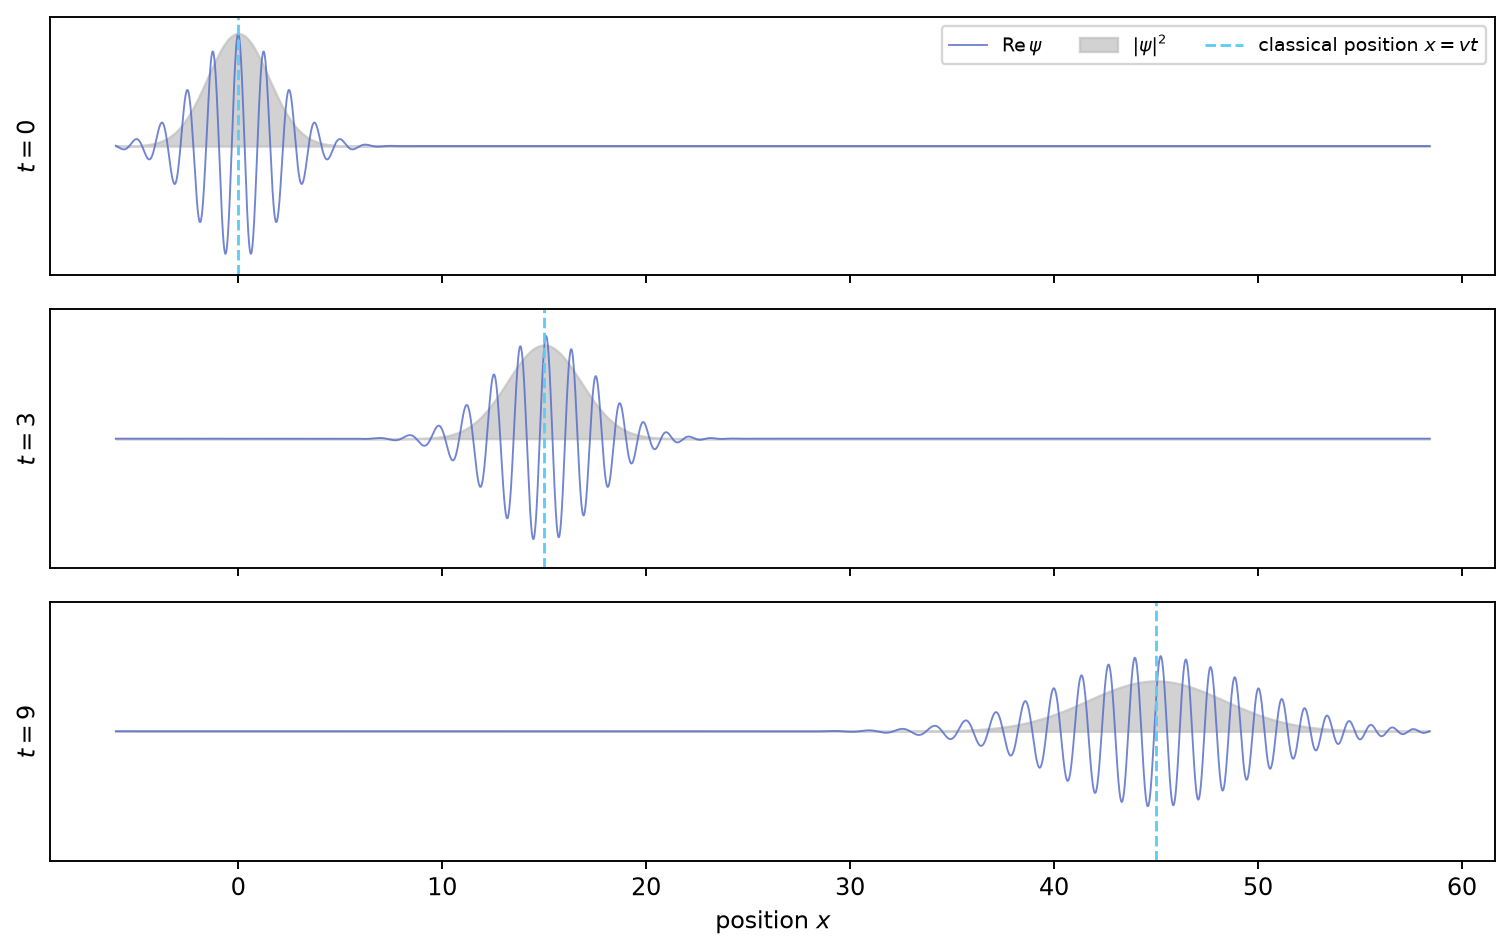
\includegraphics[width=0.95\textwidth]{figures/packet-times.png}
\caption{A Gaussian packet with $k_0=5$ and $\sigma_x=1.5$ (units with $\hbar=m=1$) at three times. Grey: probability; blue: real part of the amplitude (the individual waves inside the lump); dashed: classical position $x=vt$.}
\end{figure}

\subsection{When is a particle classical?}

A particle behaves classically if it travels far, compared with its own size, before spreading matters. The distance traveled in time $t_s$ is $vt_s=2k_0\sigma_x^2$, so
\[
\frac{vt_s}{\sigma_x}=2k_0\sigma_x,\qquad k_0\sigma_x=\frac{p_0\sigma_x}{\hbar}=\frac{p_0}{2\Delta p}.
\]
The single number $k_0\sigma_x$ is large exactly when the momentum is known to a small fraction of itself. When $k_0\sigma_x\gg1$ the lump contains many wavelengths and travels many widths before spreading, so it follows $x=vt$. When $k_0\sigma_x\sim1$ no path can be spoken of.

\begin{center}
\begin{tabular}{llll}
\hline
Particle & Localized to & $k_0\sigma_x$ & Spreading time $t_s$ \\
\hline
Electron, kinetic energy 1~eV & 1~nm & about 5 & about 17~fs \\
Dust grain, 1~mg at 1~mm/s & 1~$\mu$m & about $10^{19}$ & about $6\times10^{8}$ years \\
\hline
\end{tabular}
\end{center}

\paragraph{Numerical note.} A sum over $N$ evenly spaced values of $k$ repeats with period $2\pi/\Delta k$, so a finite sum shows copies of the lump. With Gaussian weights, about 10 components give a clean lump at $t=0$, and roughly $5\sqrt{1+(t/t_s)^2}$ are needed as it spreads; equal weights leave a sidelobe of about 5\% for any $N$. The lump width is set by the bandwidth, never by $N$.

%%%%%%%%%%%%%%%%%%%%%%%%%%%%%%%%%%%%%%%%%%%%%%%%%%%%%%%%%%%%%%%%%%%%%%%%%%%%%%%%%%%%%%%%%%%%%%%%%%%%%%%%%%%%%%%%%%%%%%%%%%%%%%%%%%%%
%% ROTATIONS
%%%%%%%%%%%%%%%%%%%%%%%%%%%%%%%%%%%%%%%%%%%%%%%%%%%%%%%%%%%%%%%%%%%%%%%%%%%%%%%%%%%%%%%%%%%%%%%%%%%%%%%%%%%%%%%%%%%%%%%%%%%%%%%%%%%%
\vfill
\eject

\section{Rotations and angular momentum}
\label{sec:rotations}

\subsection{Why study rotations}

Symmetries are tied to conserved quantities (Noether's theorem). If the physics is unchanged when everything is rotated about some axis, the component of angular momentum along that axis does not change in time. The way a quantum state transforms under rotation therefore determines what spin is.

\subsection{Rotation matrices}

In the plane, the matrix that rotates every vector through $\theta$ is
\[
R(\theta)=\begin{pmatrix}\cos\theta&-\sin\theta\\ \sin\theta&\cos\theta\end{pmatrix}.
\]
Two rotations in succession multiply their matrices; in the plane the order is immaterial ($a$ then $b$ is $a+b$). In three dimensions there is a basic rotation about each axis, for example
\[
R_z(\theta)=\begin{pmatrix}\cos\theta&-\sin\theta&0\\ \sin\theta&\cos\theta&0\\ 0&0&1\end{pmatrix},
\]
with $R_x$ and $R_y$ similar. \textbf{In three dimensions the order of rotations matters.} Rotating about $x$ then $y$ gives a different orientation than $y$ then $x$ (unless one of the angles is $0^\circ$ or $180^\circ$). This non-commutation is the only property of 3D rotations needed below. For small rotations the mismatch is exact: rotating by $\epsilon$ about $x$, then $y$, then back about $x$ and back about $y$ gives approximately a rotation by $\epsilon^2$ about $z$,
\[
R_x(\epsilon)R_y(\epsilon)R_x(-\epsilon)R_y(-\epsilon)\approx R_z(\epsilon^2),
\]
the group-level form of $[J_x,J_y]=iJ_z$.

\subsection{The $J$ matrices}

For a very small angle, $R(\epsilon)\approx 1+\epsilon K$, where $K=dR/d\theta\,|_{\theta=0}$ is the derivative of the rotation matrix at zero angle. A rotation through a finite angle is many small ones,
\[
R(\theta)=\lim_{n\to\infty}\left(1+\frac{\theta}{n}K\right)^n=e^{\theta K},
\]
the matrix analogue of continuously compounded interest. Defining $J=iK$ gives
\[
R(\theta)=e^{-i\theta J}.
\]
The factor $i$ makes $J$ have real eigenvalues, as required of a quantity whose measured values are real. So \textbf{each entry of $J$ is $i$ times the derivative, at zero angle, of the corresponding entry of the rotation matrix.} For ordinary 3D vectors, $J_z=\begin{pmatrix}0&-i&0\\ i&0&0\\ 0&0&0\end{pmatrix}$ has eigenvalues $-1,0,+1$, and the same holds for $J_x$ and $J_y$, since no direction in space is special.

\subsection{Spin number and the phase $e^{-im\theta}$}

The eigenvalues of $J_z$ are the possible values $m$ of the spin component along $z$. For ordinary vectors $m=+1,0,-1$, and the system is said to have \textbf{spin 1} (the spin number $j$ is the largest $m$). Since $R=e^{-i\theta J}$, \textbf{a rotation through $\theta$ about $z$ multiplies the amplitude of the level with value $m$ by $e^{-im\theta}$.} For integer $m$ all these phases equal 1 at $\theta=2\pi$: an ordinary vector returns to itself after a full turn.

\subsection{Conservation of $m$}

Take a state of definite $m$ in a situation unchanged by rotations about $z$. Turning the state then letting it evolve gives the same result as evolving then turning. Turning the initial state multiplies it by $e^{-im\theta}$, so the evolved state, when turned, is multiplied by the same factor: evolution leaves $m$ unchanged, whatever the details of the interaction. The same argument for shifts of position and time gives momentum and energy (section~\ref{sec:planewaves}). In matrix language the statement is $[H,J]=0$, so $d\langle J\rangle/dt=i\langle[H,J]\rangle=0$.

A test: a spinning object in a magnetic field along $\hat n$ precesses about $\hat n$; the situation is unchanged by rotations about $\hat n$, so only the component of angular momentum \emph{along the field} is conserved while the others oscillate.

%%%%%%%%%%%%%%%%%%%%%%%%%%%%%%%%%%%%%%%%%%%%%%%%%%%%%%%%%%%%%%%%%%%%%%%%%%%%%%%%%%%%%%%%%%%%%%%%%%%%%%%%%%%%%%%%%%%%%%%%%%%%%%%%%%%%
%% SPIN 1/2
%%%%%%%%%%%%%%%%%%%%%%%%%%%%%%%%%%%%%%%%%%%%%%%%%%%%%%%%%%%%%%%%%%%%%%%%%%%%%%%%%%%%%%%%%%%%%%%%%%%%%%%%%%%%%%%%%%%%%%%%%%%%%%%%%%%%
\vfill
\eject

\section{Spin one-half}
\label{sec:spinhalf}

\subsection{The electron is not spin 1}

In a Stern--Gerlach experiment a beam of silver atoms (magnetic moment of a single unpaired electron) passes through a non-uniform magnetic field, which deflects each atom according to its spin component along the field. A spin-1 system would give three beams. Experimentally \textbf{exactly two beams emerge}, for any orientation of the magnet. The electron's state has two amplitudes.

Three separate statements are involved, and only the first can be addressed with rotations:
\begin{enumerate}
    \item \textbf{Which spins can exist.} Rotation symmetry, together with the unobservability of the overall sign of a state, allows $j=0,\tfrac12,1,\tfrac32,\dots$ Half-integer spin is \emph{permitted}; experiment shows that nature uses it.
    \item \textbf{Half-integer spin implies a fermion.} This is the spin-statistics theorem (section~\ref{sec:statistics}); it does not follow from rotation symmetry alone.
    \item \textbf{Consequences.} The exclusion principle produces atomic shells and chemistry.
\end{enumerate}

\subsection{A model with two amplitudes}

The smallest model has two amplitudes of unit size, with relative phase $\phi$ and common phase $\gamma$:
\[
a_1=e^{i(\gamma-\phi/2)},\qquad a_2=e^{i(\gamma+\phi/2)}.
\]
Combining the two as in section~\ref{sec:amplitudes}, $P=\cos^2(\phi/2)$, independent of $\gamma$. Two descriptions $(\gamma,\phi)$ give the same pair $(a_1,a_2)$ also when related by $(\gamma,\phi)\to(\gamma+\pi,\phi+2\pi)$: advancing $\phi$ by $2\pi$ flips the sign of the pair, as does advancing $\gamma$ by $\pi$.

\paragraph{The value of $m$.} The observable quantity is the relative phase $\phi$: the direction of the arrow $a_1^*a_2=e^{i\phi}$ (for the electron, the direction of the spin in the $xy$-plane). A rotation of space through $\alpha$ must advance it by exactly $\alpha$. If the rotation multiplies the two amplitudes by $e^{\mp im\alpha}$, then $\phi$ advances by $2m\alpha$, so $2m=1$ and
\[
m=\pm\tfrac12.
\]
The amplitudes are the square root of the observable arrow. In a two-dimensional world the same argument allows any real $m$ (such particles are called anyons); restricting $m$ to integers and half-integers needs the non-commutation of 3D rotations.

\subsection{The matrices}

With $m=\pm\tfrac12$, a rotation through $\theta$ about $z$ multiplies the two amplitudes by $e^{\mp i\theta/2}$:
\[
U_z(\theta)=\begin{pmatrix}e^{-i\theta/2}&0\\0&e^{i\theta/2}\end{pmatrix}.
\]
The rotations about $x$ and $y$ are the $2\times2$ matrices that multiply in the same way as the ordinary rotations:
\[
U_x(\theta)=\begin{pmatrix}\cos\frac\theta2&-i\sin\frac\theta2\\-i\sin\frac\theta2&\cos\frac\theta2\end{pmatrix},\qquad
U_y(\theta)=\begin{pmatrix}\cos\frac\theta2&-\sin\frac\theta2\\ \sin\frac\theta2&\cos\frac\theta2\end{pmatrix}.
\]
Obtaining $J=iK$ exactly as before gives $J_x,J_y,J_z$ equal to the \textbf{Pauli matrices divided by 2}. These matrices turn the state through $\theta$; some texts turn the coordinate axes instead, which replaces each matrix by its inverse and writes $e^{+i\theta J}$. The physics is identical.

\subsection{A $2\pi$ rotation changes the sign}

With $m=\pm\tfrac12$ a rotation through $2\pi$ multiplies both amplitudes by $e^{\mp i\pi}=-1$ (for integer $m$, by $1$). By section~\ref{sec:amplitudes} this alters no probability of the rotated state on its own; it is detected by splitting a beam, rotating one part through $\theta$, and recombining. For spin~1 the detection probability repeats every $2\pi$; for spin~$\tfrac12$ it repeats only every $4\pi$.

\subsection{Two matrices for every rotation}

Because a state and its negative are indistinguishable by themselves, a rotation cannot tell $U$ from $-U$: \textbf{every rotation has two valid $2\times2$ matrices.} Writing $(a,b)=(\cos\frac\varphi2,\sin\frac\varphi2)$, the matrix $U_z=\mathrm{diag}(a-ib,\,a+ib)$ traces a circle with one full circuit per $4\pi$, while the ordinary $3\times3$ rotation it implements repeats every $2\pi$. At $\varphi=2\pi$, $R$ is the identity while $U=-1$. The map from $2\times2$ matrices to $3\times3$ rotations is two-to-one: these are the groups SU(2) and SO(3), and SU(2) is the \emph{double cover} of SO(3). The correspondence is
\[
R_{ij}=\tfrac12\operatorname{Tr}\!\big(\sigma_i\,U\,\sigma_j\,U^\dagger\big),
\]
where $\sigma_i=2J_i$ are the Pauli matrices; it is identical for $U$ and $-U$.

%%%%%%%%%%%%%%%%%%%%%%%%%%%%%%%%%%%%%%%%%%%%%%%%%%%%%%%%%%%%%%%%%%%%%%%%%%%%%%%%%%%%%%%%%%%%%%%%%%%%%%%%%%%%%%%%%%%%%%%%%%%%%%%%%%%%
%% BELT TRICK
%%%%%%%%%%%%%%%%%%%%%%%%%%%%%%%%%%%%%%%%%%%%%%%%%%%%%%%%%%%%%%%%%%%%%%%%%%%%%%%%%%%%%%%%%%%%%%%%%%%%%%%%%%%%%%%%%%%%%%%%%%%%%%%%%%%%

\section{The belt trick: a picture of the $4\pi$ rotation}

The sign change can be seen as a shape. A belt joins a fixed wall to a plate that is turned about the vertical axis. At each point along the belt the cross-section has an \emph{orientation}; at the wall it is the identity and at the plate it is the rotation through the angle $\varphi$ by which the plate has been turned. The belt is a continuous path of orientations from the identity to the plate's orientation. (The explicit family of belts used for the figures is given by unit quaternions, which are the $2\times2$ matrices above: $U=w-i(x\sigma_x+y\sigma_y+z\sigma_z)$.)

\begin{figure}[h]
\centering
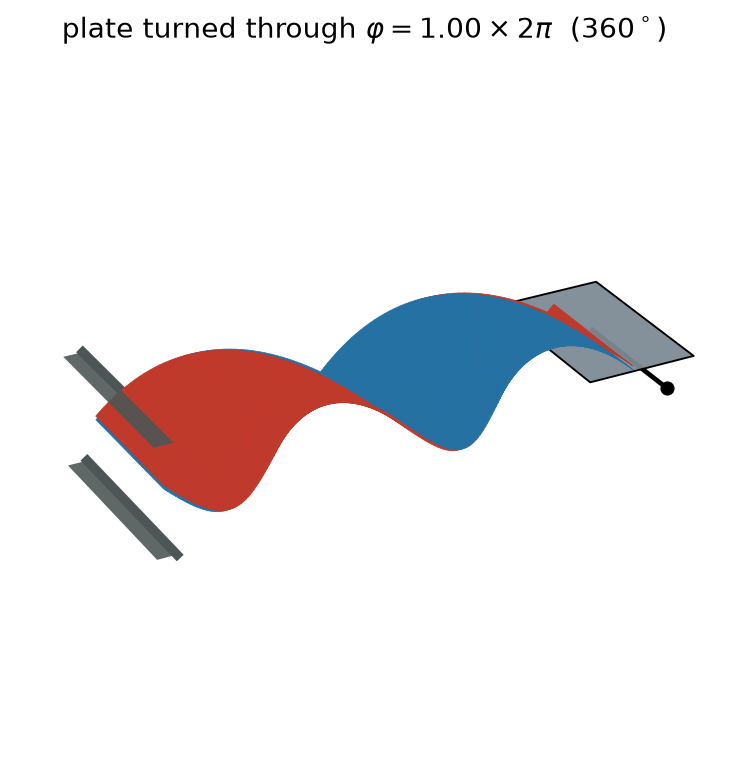
\includegraphics[width=0.46\textwidth]{figures/belt-2pi.png}\hfill
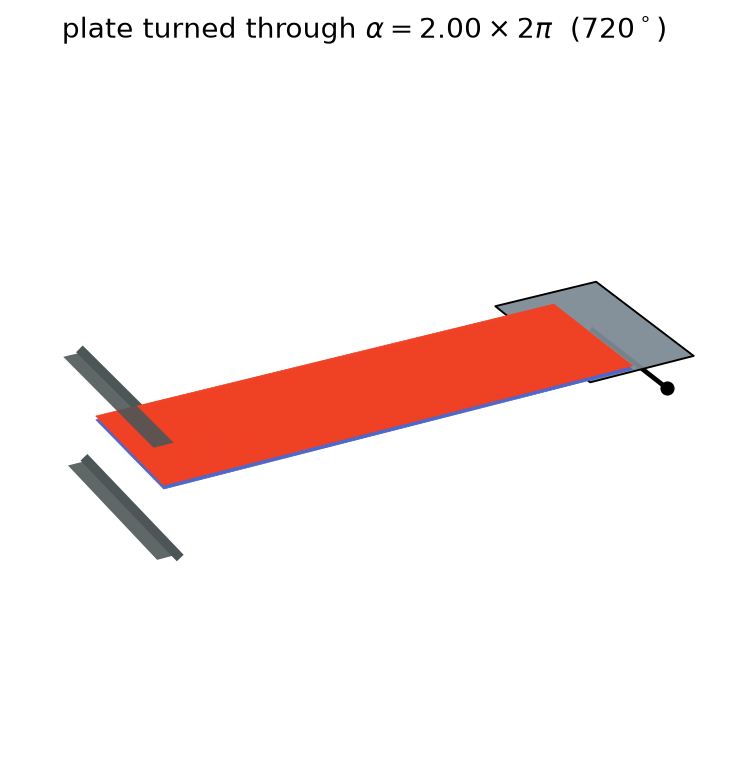
\includegraphics[width=0.46\textwidth]{figures/belt-4pi.png}
\caption{The belt after the plate has turned through $2\pi$ (left: the plate faces as it started, but the belt carries one full twist) and through $4\pi$ (right: the twist has gone and the belt is flat again). The red and blue sides are the two faces of the belt.}
\end{figure}

\begin{itemize}
    \item At $\varphi=2\pi$ the plate is back in its starting orientation but the belt is not: it has one full twist. The orientation of the plate says only that it faces as it did; the belt also records that a full turn has been made.
    \item Turning further does not add a second twist. The belt untwists, and at $4\pi$ plate and belt are both as they started.
    \item No smooth way of turning the plate leaves the belt flat at both $\varphi=0$ and $\varphi=2\pi$, but for $4\pi$ there is one.
\end{itemize}

\paragraph{The same fact as the spinor sign.} Following the belt from the wall, where $U=1$, fixes a continuous choice of sign for $U$. At the plate this is the electron's matrix $U_z(\varphi)$: $-1$ at $2\pi$, $+1$ at $4\pi$. A belt with one twist is the picture of the sign $-1$; an untwisted belt is $+1$.

\paragraph{Caveat.} The model is a family of frames (the centre line follows the cross-section's axis), so the plate is carried round a loop as the belt curls. It is not a self-avoiding belt with both ends pinned in position.

\subsection{The space of rotations as a ball}

Every orientation is a rotation through some angle in $[0,\pi]$ about some axis, so it can be drawn as a point in a ball of radius $\pi$: direction from the centre is the axis, distance is the angle, the centre is the identity. Rotations through $\pi$ about opposite axes are the same, so \textbf{opposite points on the surface are identified}: a path leaving the ball at one point continues from the opposite one.

Turning the plate about the vertical moves its orientation straight up from the centre, out of the surface at $\varphi=\pi$, back in from the opposite point, and to the centre at $2\pi$: a closed path crossing the surface once. Turning through $4\pi$ crosses the surface twice. A deformation of a closed path can create or remove crossings only in \emph{pairs} (two can merge and cancel), so a lone crossing can never disappear. Hence the $2\pi$ path can never be shrunk to the centre and the $4\pi$ path can.

\begin{figure}[h]
\centering
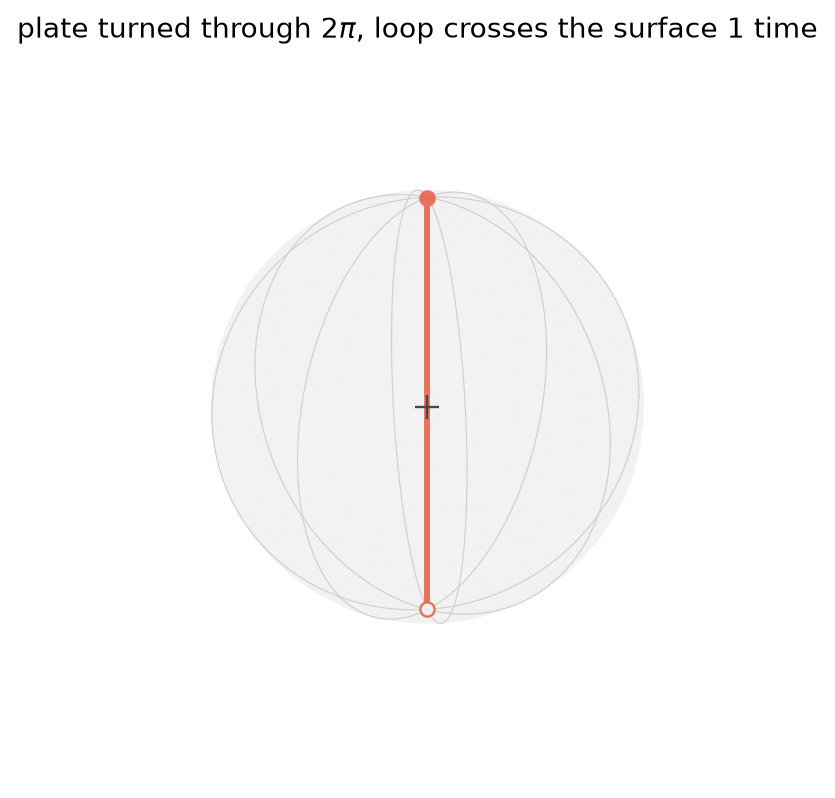
\includegraphics[width=0.46\textwidth]{figures/ball-2pi.png}\hfill
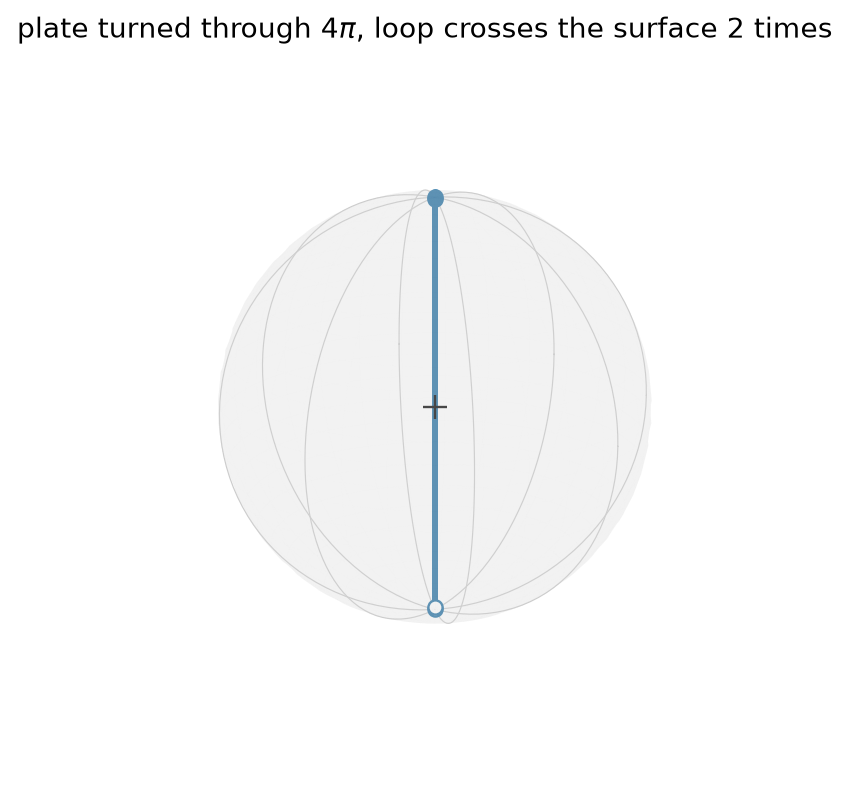
\includegraphics[width=0.46\textwidth]{figures/ball-4pi.png}
\caption{The plate's orientation as a path in the ball of rotations. Left: $2\pi$, one surface crossing, cannot be shrunk. Right: $4\pi$ (shown partly shrunk), two crossings that approach and cancel, after which the path contracts to a point.}
\end{figure}

In terms of the matrices: the $4\pi$ path lifts to a closed path of $U$ (it ends at $U=+1$) and can be shrunk; the $2\pi$ path lifts to a path from $U=+1$ to $U=-1$, which is not closed.

%%%%%%%%%%%%%%%%%%%%%%%%%%%%%%%%%%%%%%%%%%%%%%%%%%%%%%%%%%%%%%%%%%%%%%%%%%%%%%%%%%%%%%%%%%%%%%%%%%%%%%%%%%%%%%%%%%%%%%%%%%%%%%%%%%%%
%% STATISTICS
%%%%%%%%%%%%%%%%%%%%%%%%%%%%%%%%%%%%%%%%%%%%%%%%%%%%%%%%%%%%%%%%%%%%%%%%%%%%%%%%%%%%%%%%%%%%%%%%%%%%%%%%%%%%%%%%%%%%%%%%%%%%%%%%%%%%
\vfill
\eject

\section{Bosons, fermions, and what rotations do not tell us}
\label{sec:statistics}

All known particles fall into two classes, distinguished by two related properties:

\begin{itemize}
    \item \textbf{Rotation.} The state of a boson is unchanged by a $2\pi$ rotation; the state of a fermion changes sign, and $4\pi$ restores it. Bosons have integer spin, fermions half-integer spin.
    \item \textbf{Exchange.} Interchanging two identical bosons leaves the joint state unchanged (symmetric); interchanging two identical fermions changes its sign (antisymmetric).
\end{itemize}

Bosons (photons, for example) can occupy the same quantum state in any number. Fermions (electrons, protons, neutrons) cannot: this is the \textbf{Pauli exclusion principle}, which gives atoms their shell structure and underlies chemistry.

\paragraph{What rotation symmetry gives.} That half-integer spin is allowed, and that it brings a sign change at $2\pi$.

\paragraph{What it does not give.} That half-integer spin means fermion. This link between rotation and exchange is the \emph{spin-statistics theorem} (Pauli, 1940), proved in relativistic quantum field theory from Lorentz invariance, locality, and positive energy. A heuristic: exchanging two particles resembles a half-turn of the pair, which would contribute the sign $(-1)^{2j}$ found above for a $2\pi$ rotation. Rigorous proofs are considerably more demanding. Exchange itself follows the pattern of the reflection example in section~\ref{sec:amplitudes}: applying it twice restores the state, so exchange multiplies the joint state by $+1$ or $-1$.

%%%%%%%%%%%%%%%%%%%%%%%%%%%%%%%%%%%%%%%%%%%%%%%%%%%%%%%%%%%%%%%%%%%%%%%%%%%%%%%%%%%%%%%%%%%%%%%%%%%%%%%%%%%%%%%%%%%%%%%%%%%%%%%%%%%%
%% TECHNICAL
%%%%%%%%%%%%%%%%%%%%%%%%%%%%%%%%%%%%%%%%%%%%%%%%%%%%%%%%%%%%%%%%%%%%%%%%%%%%%%%%%%%%%%%%%%%%%%%%%%%%%%%%%%%%%%%%%%%%%%%%%%%%%%%%%%%%

\section{Technical notes}

These are the more advanced versions of arguments made above. They need linear algebra and some group theory.

\subsection{Quantization of $m$ from commutators}

Non-commutation gives $J_z=-i[J_x,J_y]$ and, with $J_\pm=J_x\pm iJ_y$,
\[
[J_z,J_\pm]=\pm J_\pm .
\]
If $J_z|m\rangle=m|m\rangle$, then $J_+|m\rangle$ has $J_z$-eigenvalue exactly $m+1$ and $J_-|m\rangle$ has $m-1$: the values of $m$ come in steps of 1. In a finite number of states the ladder must stop at a top state ($J_+|m_{\max}\rangle=0$) and a bottom state ($J_-|m_{\min}\rangle=0$). Since $\|J_\pm|m\rangle\|^2=j(j+1)-m(m\pm1)$, vanishing at the ends forces $m_{\min}=-m_{\max}\equiv-j$, and $N$ steps of 1 from $-j$ to $+j$ give $2j=N-1$, an integer. The commutator loop above is the same for every spin (the error against $R_z(\epsilon^2)$ shrinks like $\epsilon^3$), so the non-commuting structure is representation-independent and $j$ labels which representation one has.

\subsection{Neighboring levels differ by one}

A heuristic version without commutators: the spin direction is set by products of amplitudes of neighboring levels, with relative phase $e^{i(m_1-m_2)\theta}$ under a rotation by $\theta$. This phase must equal the geometric angle $\theta$ of the spin direction, so the spacing is exactly 1. Rotating $180^\circ$ about $y$ interchanges up and down, so the set of $m$ is symmetric about zero. For $N$ levels, $j=(N-1)/2$, and the effect of a $2\pi$ rotation is
\begin{center}
\begin{tabular}{llll}
\hline
$N$ levels & $j$ & $m$ values & $2\pi$ rotation \\
\hline
1 & 0 & 0 & unchanged \\
2 & $\tfrac12$ & $\pm\tfrac12$ & sign change \\
3 & 1 & $-1,0,+1$ & unchanged \\
4 & $\tfrac32$ & $\pm\tfrac12,\pm\tfrac32$ & sign change \\
\hline
\end{tabular}
\end{center}
An even number of levels always produces a sign change. The first guess for two levels, $m=\pm1$, fails: at $\phi=\pi$ both amplitudes get $-1$ (an unobservable common sign), so $+x$ never becomes $-x$.

\subsection{Noether's theorem in quantum mechanics}

The generator in $U(\hat n,\theta)=e^{-i\theta\,\hat n\cdot\mathbf J}$ is $\mathbf J$ itself. If $H$ is rotationally invariant, $UHU^\dagger=H$ for every rotation, and expanding to first order in $\theta$ gives $[H,\hat n\cdot\mathbf J]=0$. The Heisenberg equation then gives
\[
\frac{d\langle\mathbf J\rangle}{dt}=i\langle[H,\mathbf J]\rangle=0.
\]
The conserved quantity is literally the generator of the symmetry. A magnetic field breaks rotation symmetry but $H=\omega\,\hat n\cdot\mathbf J$ is still invariant under rotations about $\hat n$, so only $\hat n\cdot\mathbf J$ is conserved and the other components precess.

\subsection{Projective representations and the double cover}

Quantum states are rays, so symmetry only requires $U(\text{rot}_2)U(\text{rot}_1)=\pm U(\text{rot}_2\circ\text{rot}_1)$. SO(3) is not simply connected ($\pi_1=\mathbb{Z}_2$): a $2\pi$ rotation is a loop that cannot be shrunk to a point, but a $4\pi$ loop can. Its projective representations are therefore exactly the ordinary representations of its simply connected double cover, SU(2), which is where half-integer spins come from; the belt trick shows the loop. The relativistic analogue is the double cover $SL(2,\mathbb{C})$ of the Lorentz group, which is where Weyl and Dirac spinors live.

\subsection{Why the groups matter in practice}

Equivariant machine-learned force fields (see the force fields notes) are built on exactly this representation theory: features are labeled by $j$ (angular momentum order), and rotating the input molecule acts on them by the matrices above. A rotation of the molecule must rotate energies trivially and forces as vectors; the spin-1 representation is the force.

% TODO: connect to electronic-structure methods (Hartree--Fock, DFT) once those notes exist: antisymmetry of the electronic wave function (Slater determinants) is the exchange rule above.

\end{document}
